\begin{question}
\noindent An engineer models the orientation of a triangular satellite dish panel, $T$, on a coordinate grid, where each unit represents 1 metre. The panel has vertices $A(1,1)$, $B(1,3)$ and $C(2,1)$.

\noindent To redirect the signal path, the panel is first \textbf{reflected in the $y$-axis} to give panel $T_1$, and then $T_1$ is \textbf{rotated $90^\circ$ clockwise about the origin} to give panel $T_2$.

\begin{center}
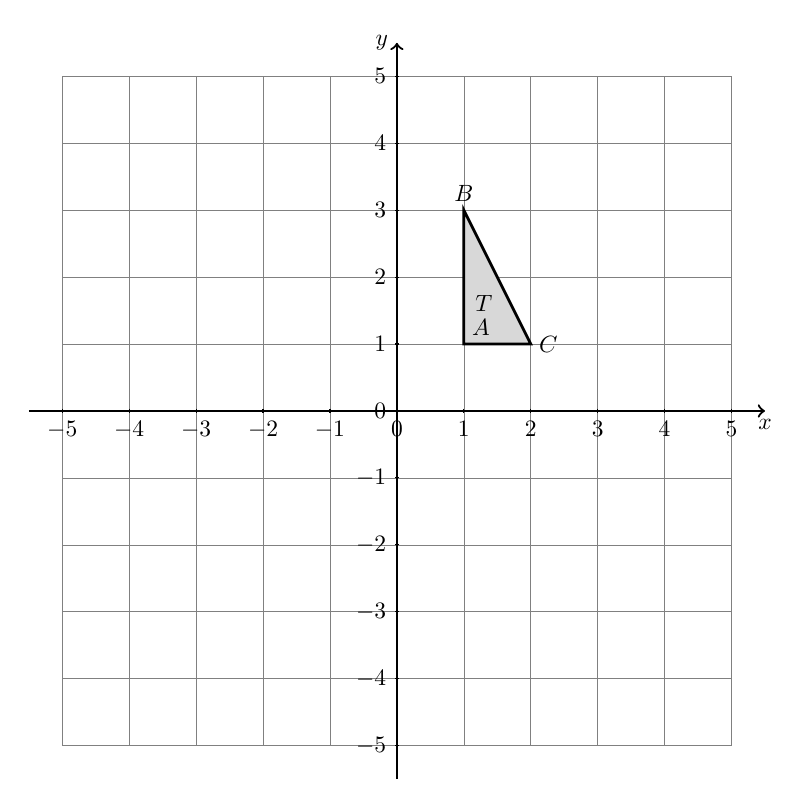
\begin{tikzpicture}[scale=0.85, transform shape]
    \definecolor{borderColour}{HTML}{000000}
    \definecolor{fillColour}{HTML}{D8D8D8}

    \def\axisLimit{5}

    % Draw grid
    \draw[step=1cm,gray,very thin] (-\axisLimit,-\axisLimit) grid (\axisLimit,\axisLimit);

    % Draw axes
    \draw[thick,->] (-\axisLimit-0.5,0) -- (\axisLimit+0.5,0) node[anchor=north] {$x$};
    \draw[thick,->] (0,-\axisLimit-0.5) -- (0,\axisLimit+0.5) node[anchor=east] {$y$};

    \foreach \x in {-\axisLimit,...,\axisLimit}
        \draw (\x cm,1pt) -- (\x cm,-1pt) node[anchor=north] {$\x$};
    \foreach \y in {-\axisLimit,...,\axisLimit}
        \draw (1pt,\y cm) -- (-1pt,\y cm) node[anchor=east] {$\y$};

    % Original triangle T
    \coordinate (A) at (1,1);
    \coordinate (B) at (1,3);
    \coordinate (C) at (2,1);

    \filldraw[fill=fillColour, draw=borderColour, line width=1pt] (A) -- (B) -- (C) -- cycle;
    \node[above right] at (A) {$A$};
    \node[above] at (B) {$B$};
    \node[right] at (C) {$C$};
    \node at (1.3,1.6) {$T$};

\end{tikzpicture}
\end{center}

\begin{enumerate}
    \item[(a)] Find the coordinates of the vertices of $T_2$, the image of $T$ after both transformations have been applied in the order stated above.
    \vspace{5cm}
    \answerplain{3}

    \item[(b)] Describe fully the \textbf{single} transformation that maps $T$ directly onto $T_2$.
    \vspace{2.5cm}
    \answerplain{1}
\end{enumerate}
\end{question}
